\documentclass[12pt,a4paper,twocolumn]{article}
% The following LaTeX packages must be installed on your machine: amsmath, authblk, bm, booktabs, caption, dcolumn, fancyhdr, geometry, graphicx, hyperref, latexsym, natbib
\input{151.dat}
\usepackage{gensymb}
\usepackage{amsthm}
\usepackage{float}
\usepackage{siunitx}
\usepackage{amssymb}
\usepackage{float}
\usepackage{enumerate}
\usepackage{listings}
\usepackage{mathtools}
\PassOptionsToPackage{hyphens}{url}\usepackage{hyperref}
\usepackage[none]{hyphenat}
\usepackage{physics}
%\renewcommand{\familydefault}{\sfdefault}


\begin{document}

\setcounter{page}{1}

\section*{PS 37: Problem 4.10}
\bigskip

\begin{enumerate}[(a)]

\item For an Einstein solid of $N=20$ distinguishable particles, the total number of accessible microstates $\Omega(E)$ is given by

\begin{equation}
	\Omega(E) = \frac{\qty(E + N - 1)!}{E!\qty(N-1)!} \label{eq:accessible}
\end{equation}

For various $E$, we have

\begin{align}
	\Omega(E = 10) &= \frac{\qty(10 + 20 - 1)!}{10!\qty(20-1)!} \nonumber \\
	\Aboxed{
		\Omega(E = 10) &= 20,030,010
	} \\
	\Omega(E=100) &= \frac{\qty(100 + 20 - 1)!}{100!\qty(20-1)!} \nonumber \\
	\Aboxed{
		\Omega(E = 100) &\approx 4.91 \times 10^{21}
	} \\
	\Omega(E=1000) &= \frac{\qty(1000 + 20 - 1)!}{1000!\qty(20-1)!} \nonumber \\
	\Aboxed{
		\Omega(E = 1000) &\approx 9.93 \times 10^{39}
	} 
\end{align}

Continuing this process for larger $E$ for fixed $N$, we obtain the graph in Figure \ref{fig:microstates}.

\begin{figure}[h!]
	\centering
	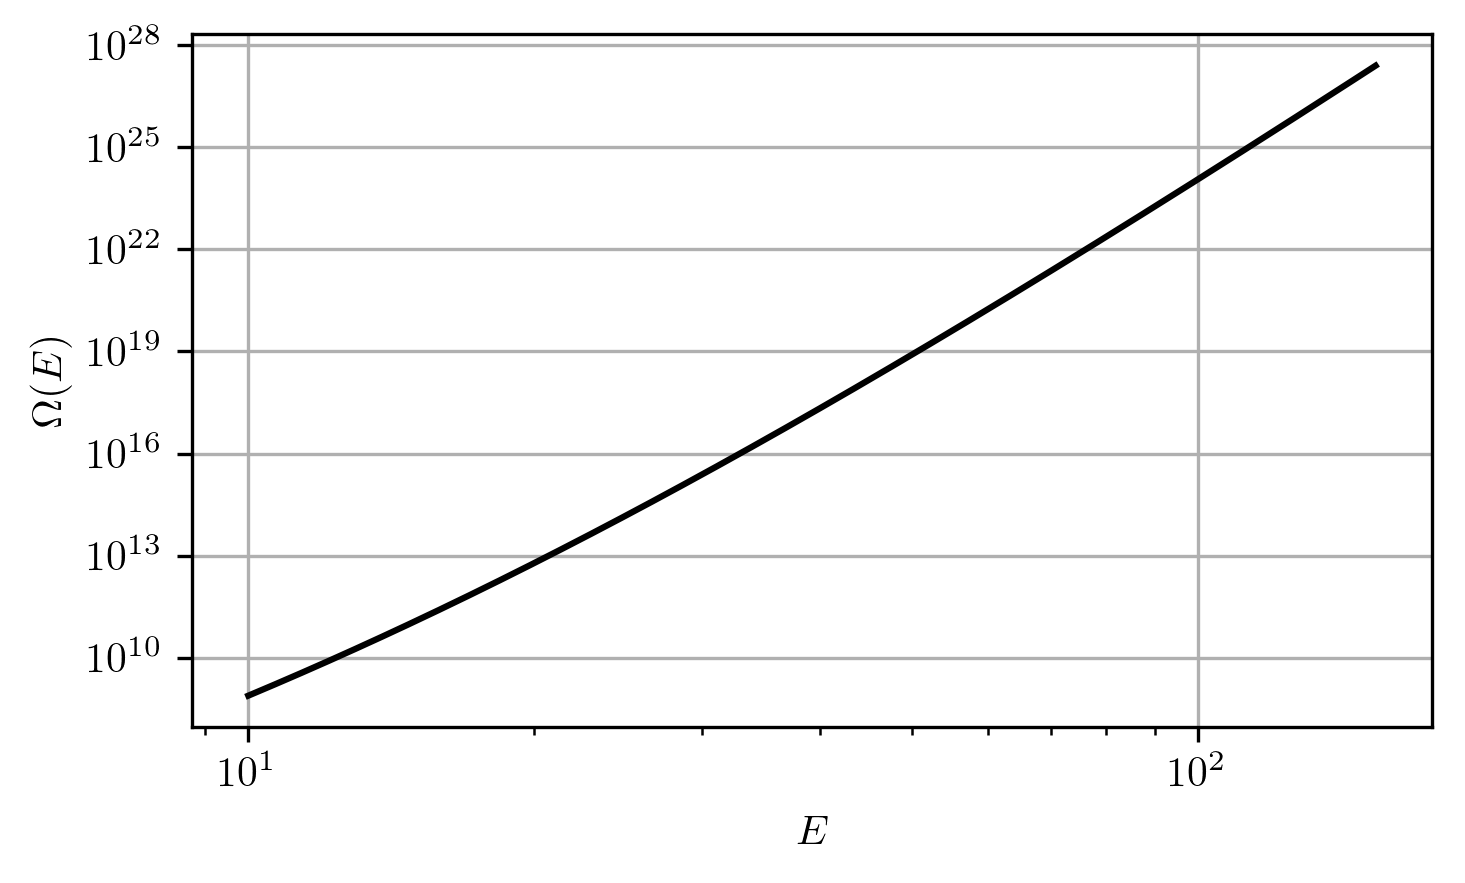
\includegraphics[width=\linewidth]{microstates.png}
	\caption{$\Omega(E) \forall E \in \qty[10^1, 10^3]$}
	\label{fig:microstates}
\end{figure}

Thus, $\Omega(E)$ is an exponentially increasing function of $E$ for fixed $N$.

\item For fixed $E = 10$ and varying $N$, we obtain the graph in Figure \ref{fig:fixed-N}.

\begin{figure}[h!]
	\centering
	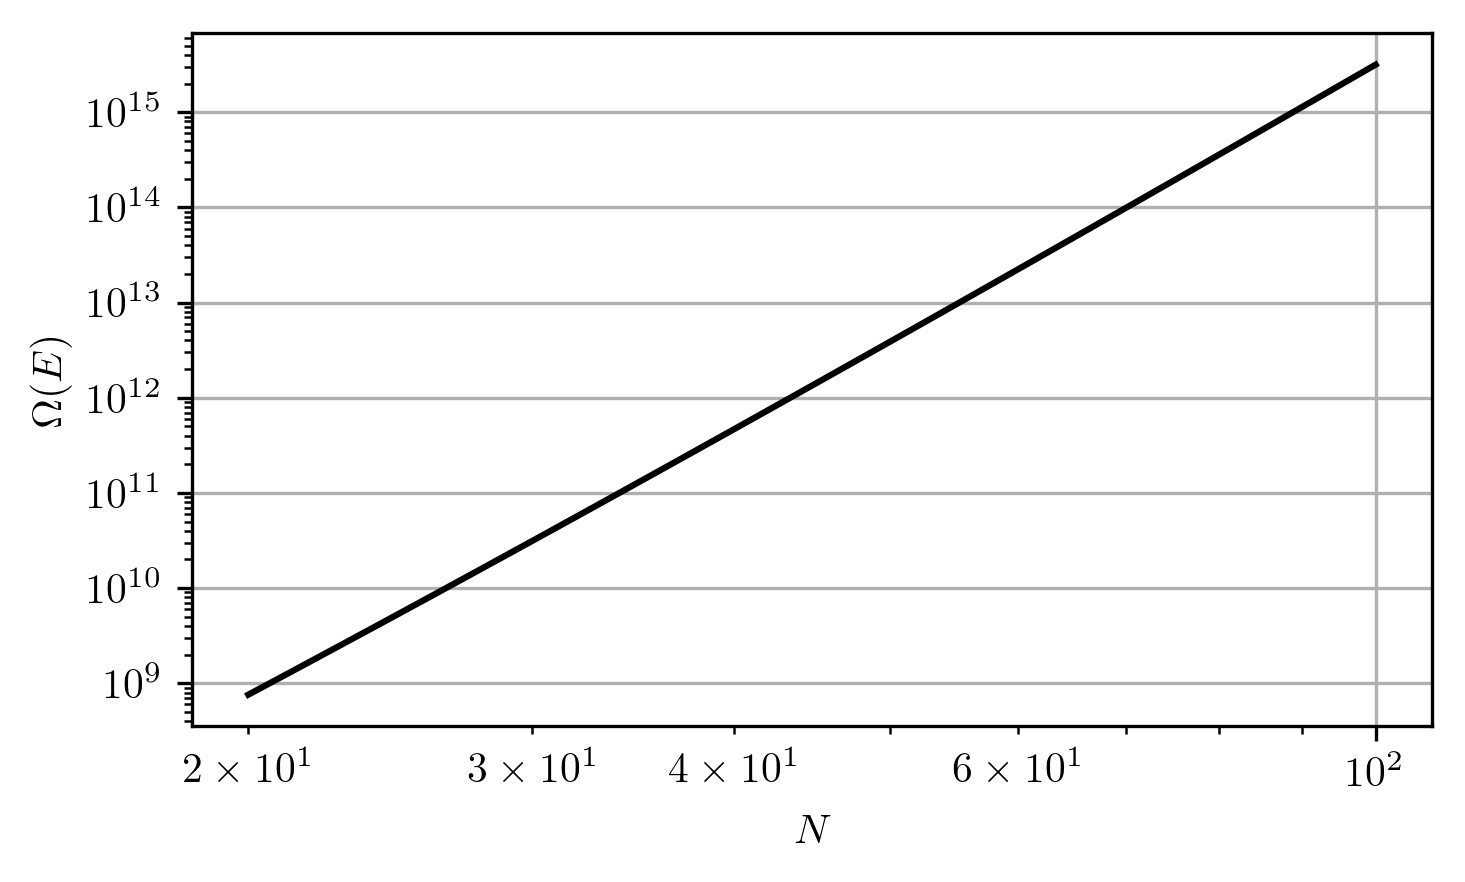
\includegraphics[width=\linewidth]{fixedN.png}
	\caption{$\Omega(E) \forall N \in \qty[20, 100]$}
	\label{fig:fixed-N}
\end{figure}

Thus, $\Omega(E)$ is also an exponentially increasing function of $N$ for fixed $E$.

\end{enumerate}

\end{document}